\chapter{Quick Revision: OE-EC804A - Artificial Intelligence}

This high-yield index contains key definitions, formulas, repeated questions, practice diagrams, and last-minute revision points to review before exams.


\section{Unit I: Introduction}

\subsection{1. Important Definitions}
\begin{itemize}
  \item   \textbf{Artificial Intelligence:} Autonomous systems performing cognitive tasks that typically require human intelligence.
  \item   \textbf{Rational Agent:} An agent that acts to achieve the best possible (or best expected) outcome based on its inputs and knowledge.
  \item   \textbf{Turing Test:} An operational test where a computer is considered intelligent if a human interrogator cannot distinguish it from a human in textual conversations.
  \item   \textbf{Expert System:} Specialized interactive software emulating a human expert's decision-making in a narrow domain.
  \item   \textbf{Inference Engine:} The reasoning logic in an Expert System that applies facts/rules to draw conclusions.
  \item   \textbf{Forward Chaining:} Data-driven reasoning starting from known facts to reach a conclusion.
  \item   \textbf{Backward Chaining:} Goal-driven reasoning starting from a hypothesis/goal to find supporting facts.
  \item   \textbf{Knowledge Acquisition Bottleneck:} The slow, difficult task of extracting human expertise into rigid computer rules.
\end{itemize}

\subsection{Key Formulas}
\textit{   }None for Unit I. (Note: Search complexities and Bayes probability formulas appear in later units).*

\subsection{Frequently Asked Questions}
\begin{enumerate}
  \item \textbf{"Describe different components of AI." [5M][]}
\end{enumerate}
    \textit{   }Core point:* Focus on NLP, Machine Learning, Computer Vision, Robotics, and Expert Systems. Include the Sensing $\rightarrow$ Reasoning $\rightarrow$ Learning $\rightarrow$ Acting functional diagram.
\begin{enumerate}
  \item \textbf{"What is an Expert System? Explain its components." [10M][]}
\end{enumerate}
    \textit{   }Core point:* Define ES. Draw the Knowledge Base $\leftrightarrow$ Inference Engine $\leftrightarrow$ User Interface block diagram. Detail forward/backward chaining. List 5 advantages and 5 disadvantages.

\subsection{Diagrams to Practice}
\begin{enumerate}
  \item \textbf{The Turing Test Setup:}
\end{enumerate}
    \begin{figure}[H]
\centering
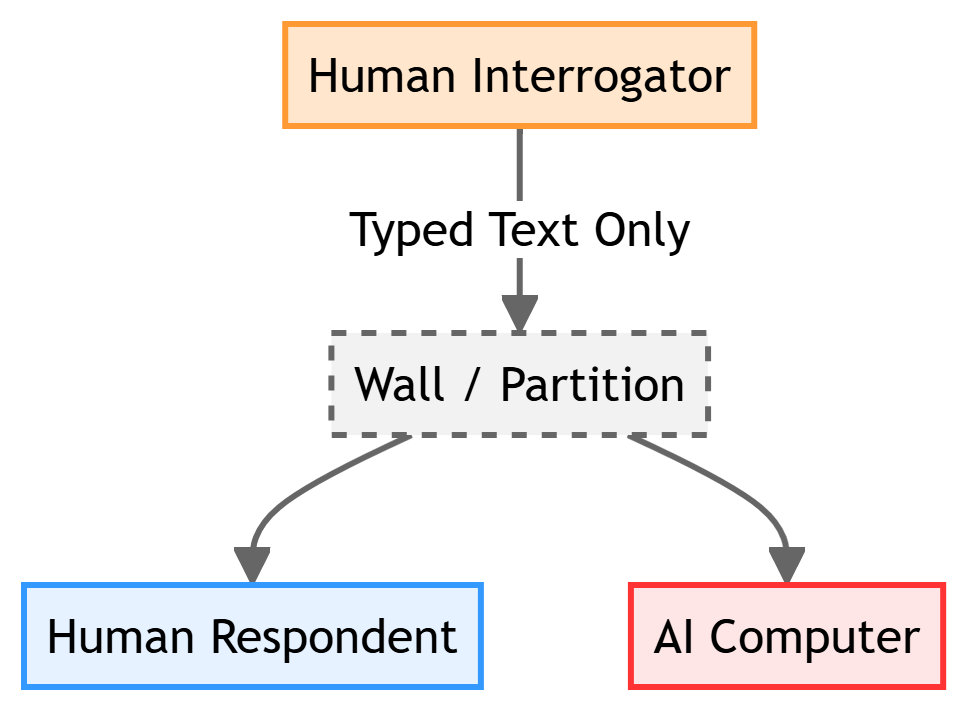
\includegraphics[width=0.75\textwidth,height=0.32\textheight,keepaspectratio]{../Images/chapter_01/turing_test_setup.png}
\caption{Turing Test Setup}
\end{figure}
\begin{enumerate}
  \item \textbf{Expert System Block Diagram:}
\end{enumerate}
    \begin{figure}[H]
\centering
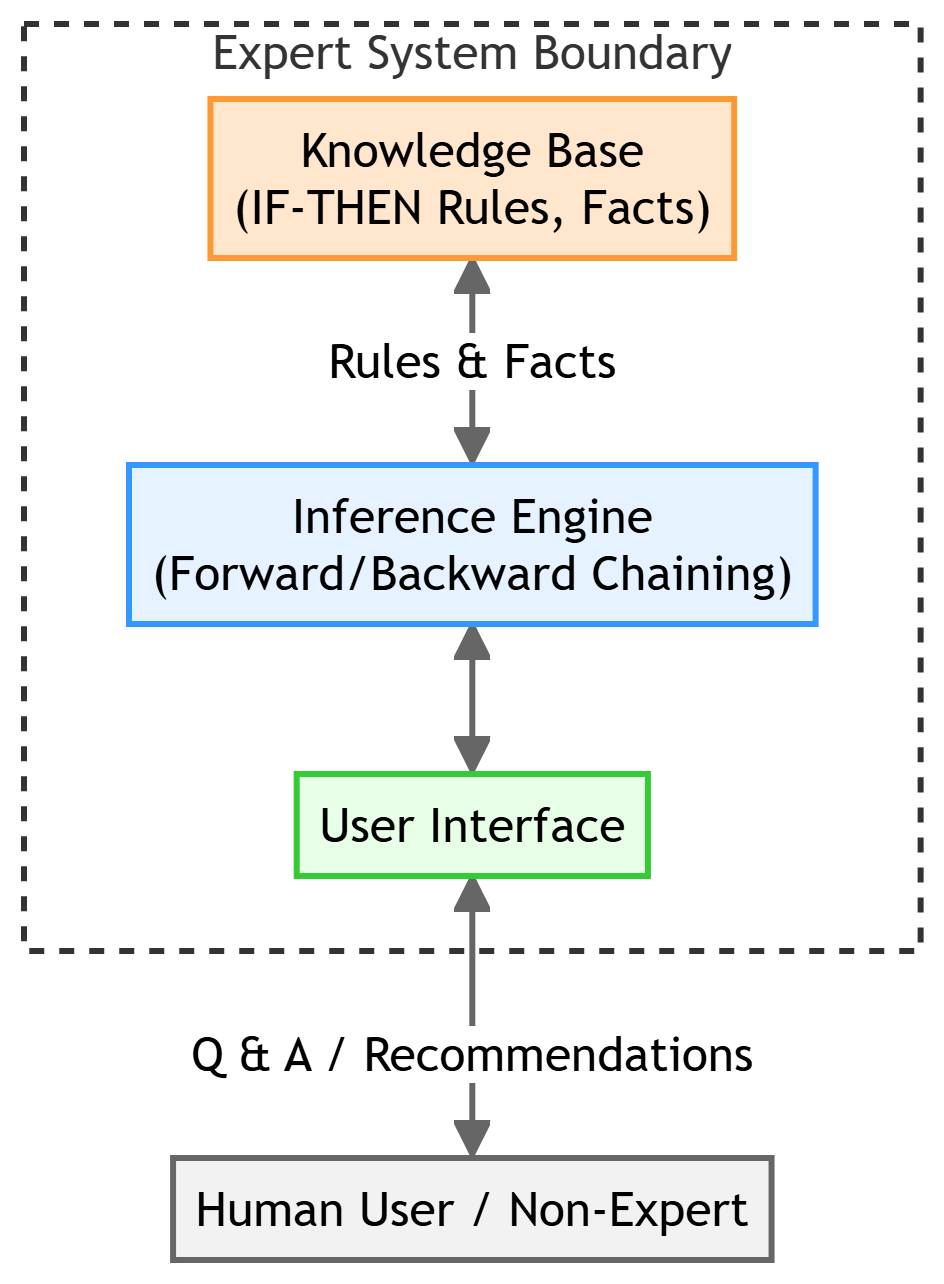
\includegraphics[width=0.75\textwidth,height=0.32\textheight,keepaspectratio]{../Images/chapter_01/expert_system_arch.png}
\caption{Expert System Architecture}
\end{figure}

\subsection{One-Line Revision}
\begin{itemize}
  \item   AI is divided into 4 views: Thinking/Acting Humanly (behavioral) and Thinking/Acting Rationally (performance-driven).
  \item   Acting Rationally (Rational Agent approach) is the standard modern paradigm of AI studies.
  \item   The Turing Test requires NLP, Knowledge Representation, Automated Reasoning, and Machine Learning.
  \item   The Total Turing Test adds Computer Vision and Robotics.
  \item   Expert Systems use rigid \textbf{IF-THEN production rules} for representation.
  \item   Forward Chaining is \textbf{data-driven}; Backward Chaining is \textbf{goal-driven}.
\end{itemize}


\section{Unit II: Intelligent Agents}

\subsection{1. Important Definitions}
\begin{itemize}
  \item   \textbf{Agent:} Anything that perceives its environment through sensors and acts upon it through actuators.
  \item   \textbf{Percept Sequence:} The complete history of all percepts received by the agent to date.
  \item   \textbf{Agent Function ($f$):} A mathematical mapping $f: P^* \rightarrow A$ from any percept sequence to an action.
  \item   \textbf{Agent Program:} The concrete implementation of the agent function running on the physical architecture.
  \item   \textbf{PEAS:} Performance measure, Environment, Actuators, Sensors. Used to specify the task environment.
  \item   \textbf{Rational Agent:} An agent that selects actions to maximize its expected performance measure given its percept history and knowledge.
  \item   \textbf{Autonomy:} An agent behaves with autonomy if its behavior is determined by its own experience rather than depending solely on built-in designer knowledge.
\end{itemize}

\subsection{Key Formulas}
\begin{itemize}
  \item   $\text{Agent} = \text{Architecture} + \text{Program}$
  \item   $f: P^* \rightarrow A$ (Agent Function mapping percept history to action)
\end{itemize}

\subsection{Frequently Asked Questions}
\begin{enumerate}
  \item \textbf{"Define PEAS description for an automated taxi driver." [5M][]}
\end{enumerate}
    \textit{   }Core point:* P: Safety, speed, comfort, profits. E: Roads, traffic, pedestrians. A: Steering, gas, brakes, display. S: Cameras, LIDAR, GPS, speedometer.
\begin{enumerate}
  \item \textbf{"Explain the five basic agent structures." [15M][]}
\end{enumerate}
    \textit{   }Core point:* Simple Reflex (percept-action rules), Model-Based (uses state to track unobserved world), Goal-Based (uses goals to plan), Utility-Based (uses utility function for state preference), Learning Agent (Critic, Learning Element, Performance Element, Problem Generator).

\subsection{Diagrams to Practice}
\begin{enumerate}
  \item \textbf{Simple Reflex and Model-Based Agents:}
\end{enumerate}
    \begin{figure}[H]
\centering
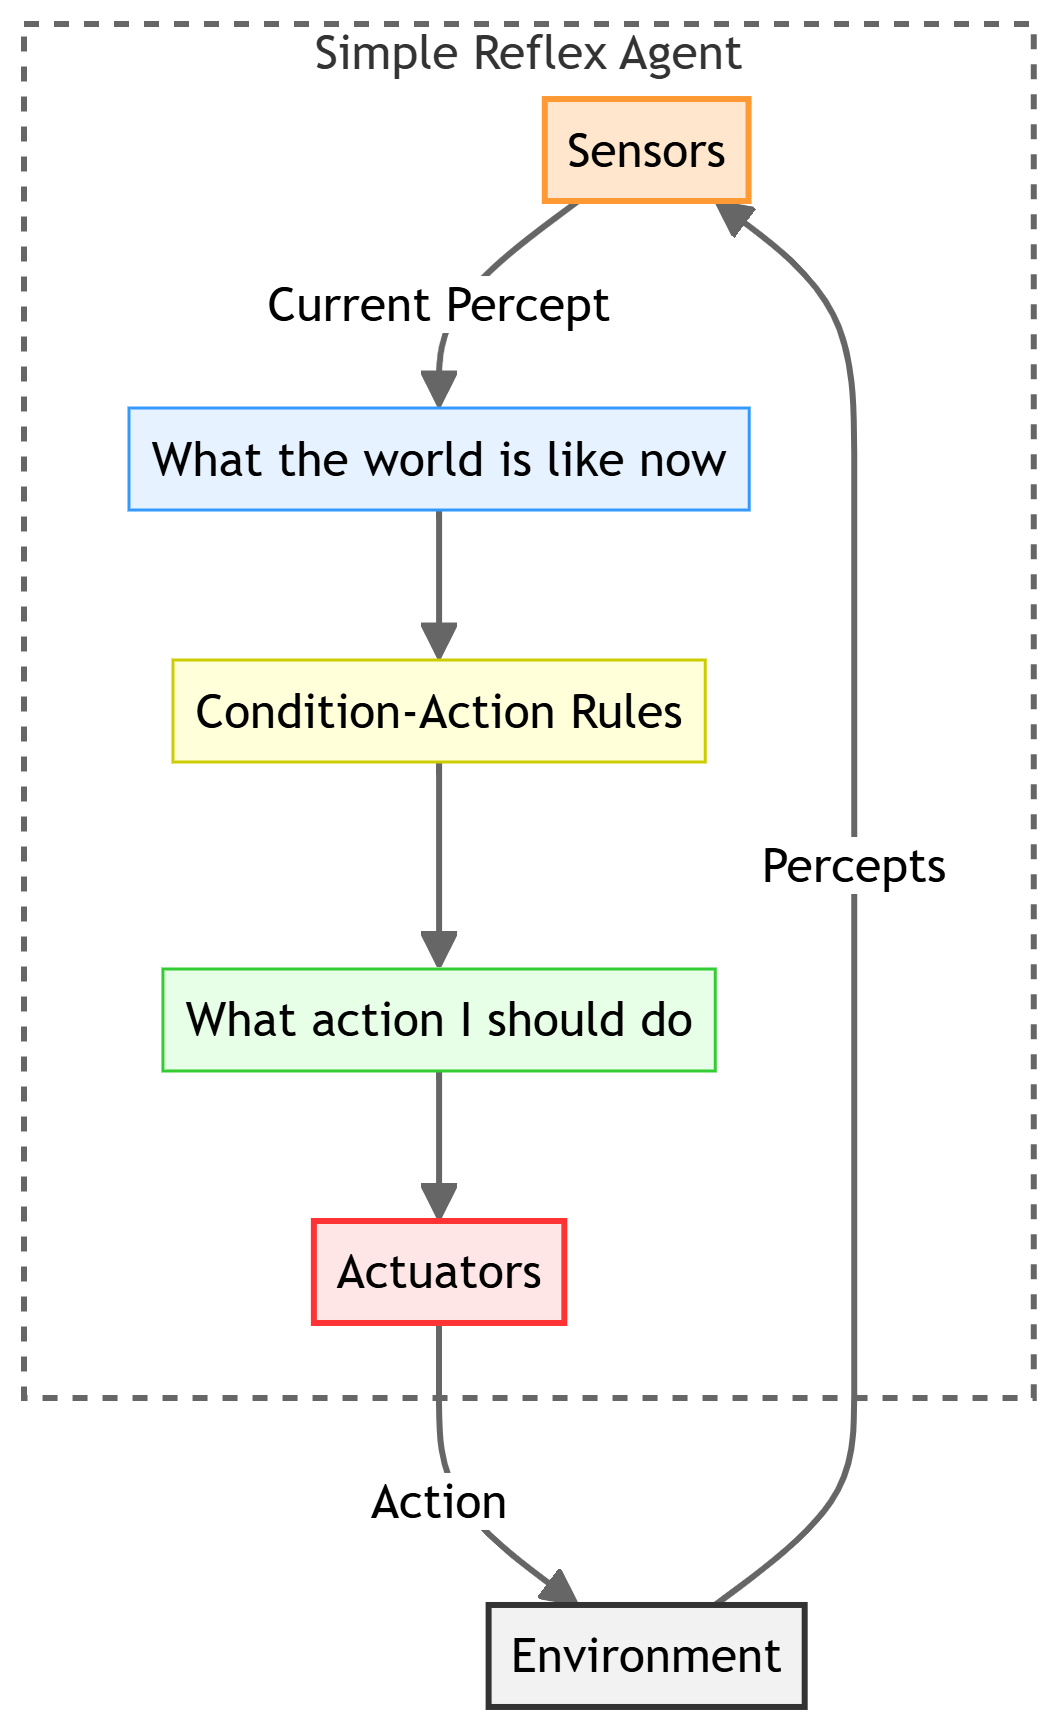
\includegraphics[width=0.75\textwidth,height=0.32\textheight,keepaspectratio]{../Images/chapter_02/simple_reflex_agent.png}
\caption{Simple Reflex Agent Structure}
\end{figure}
    \begin{figure}[H]
\centering
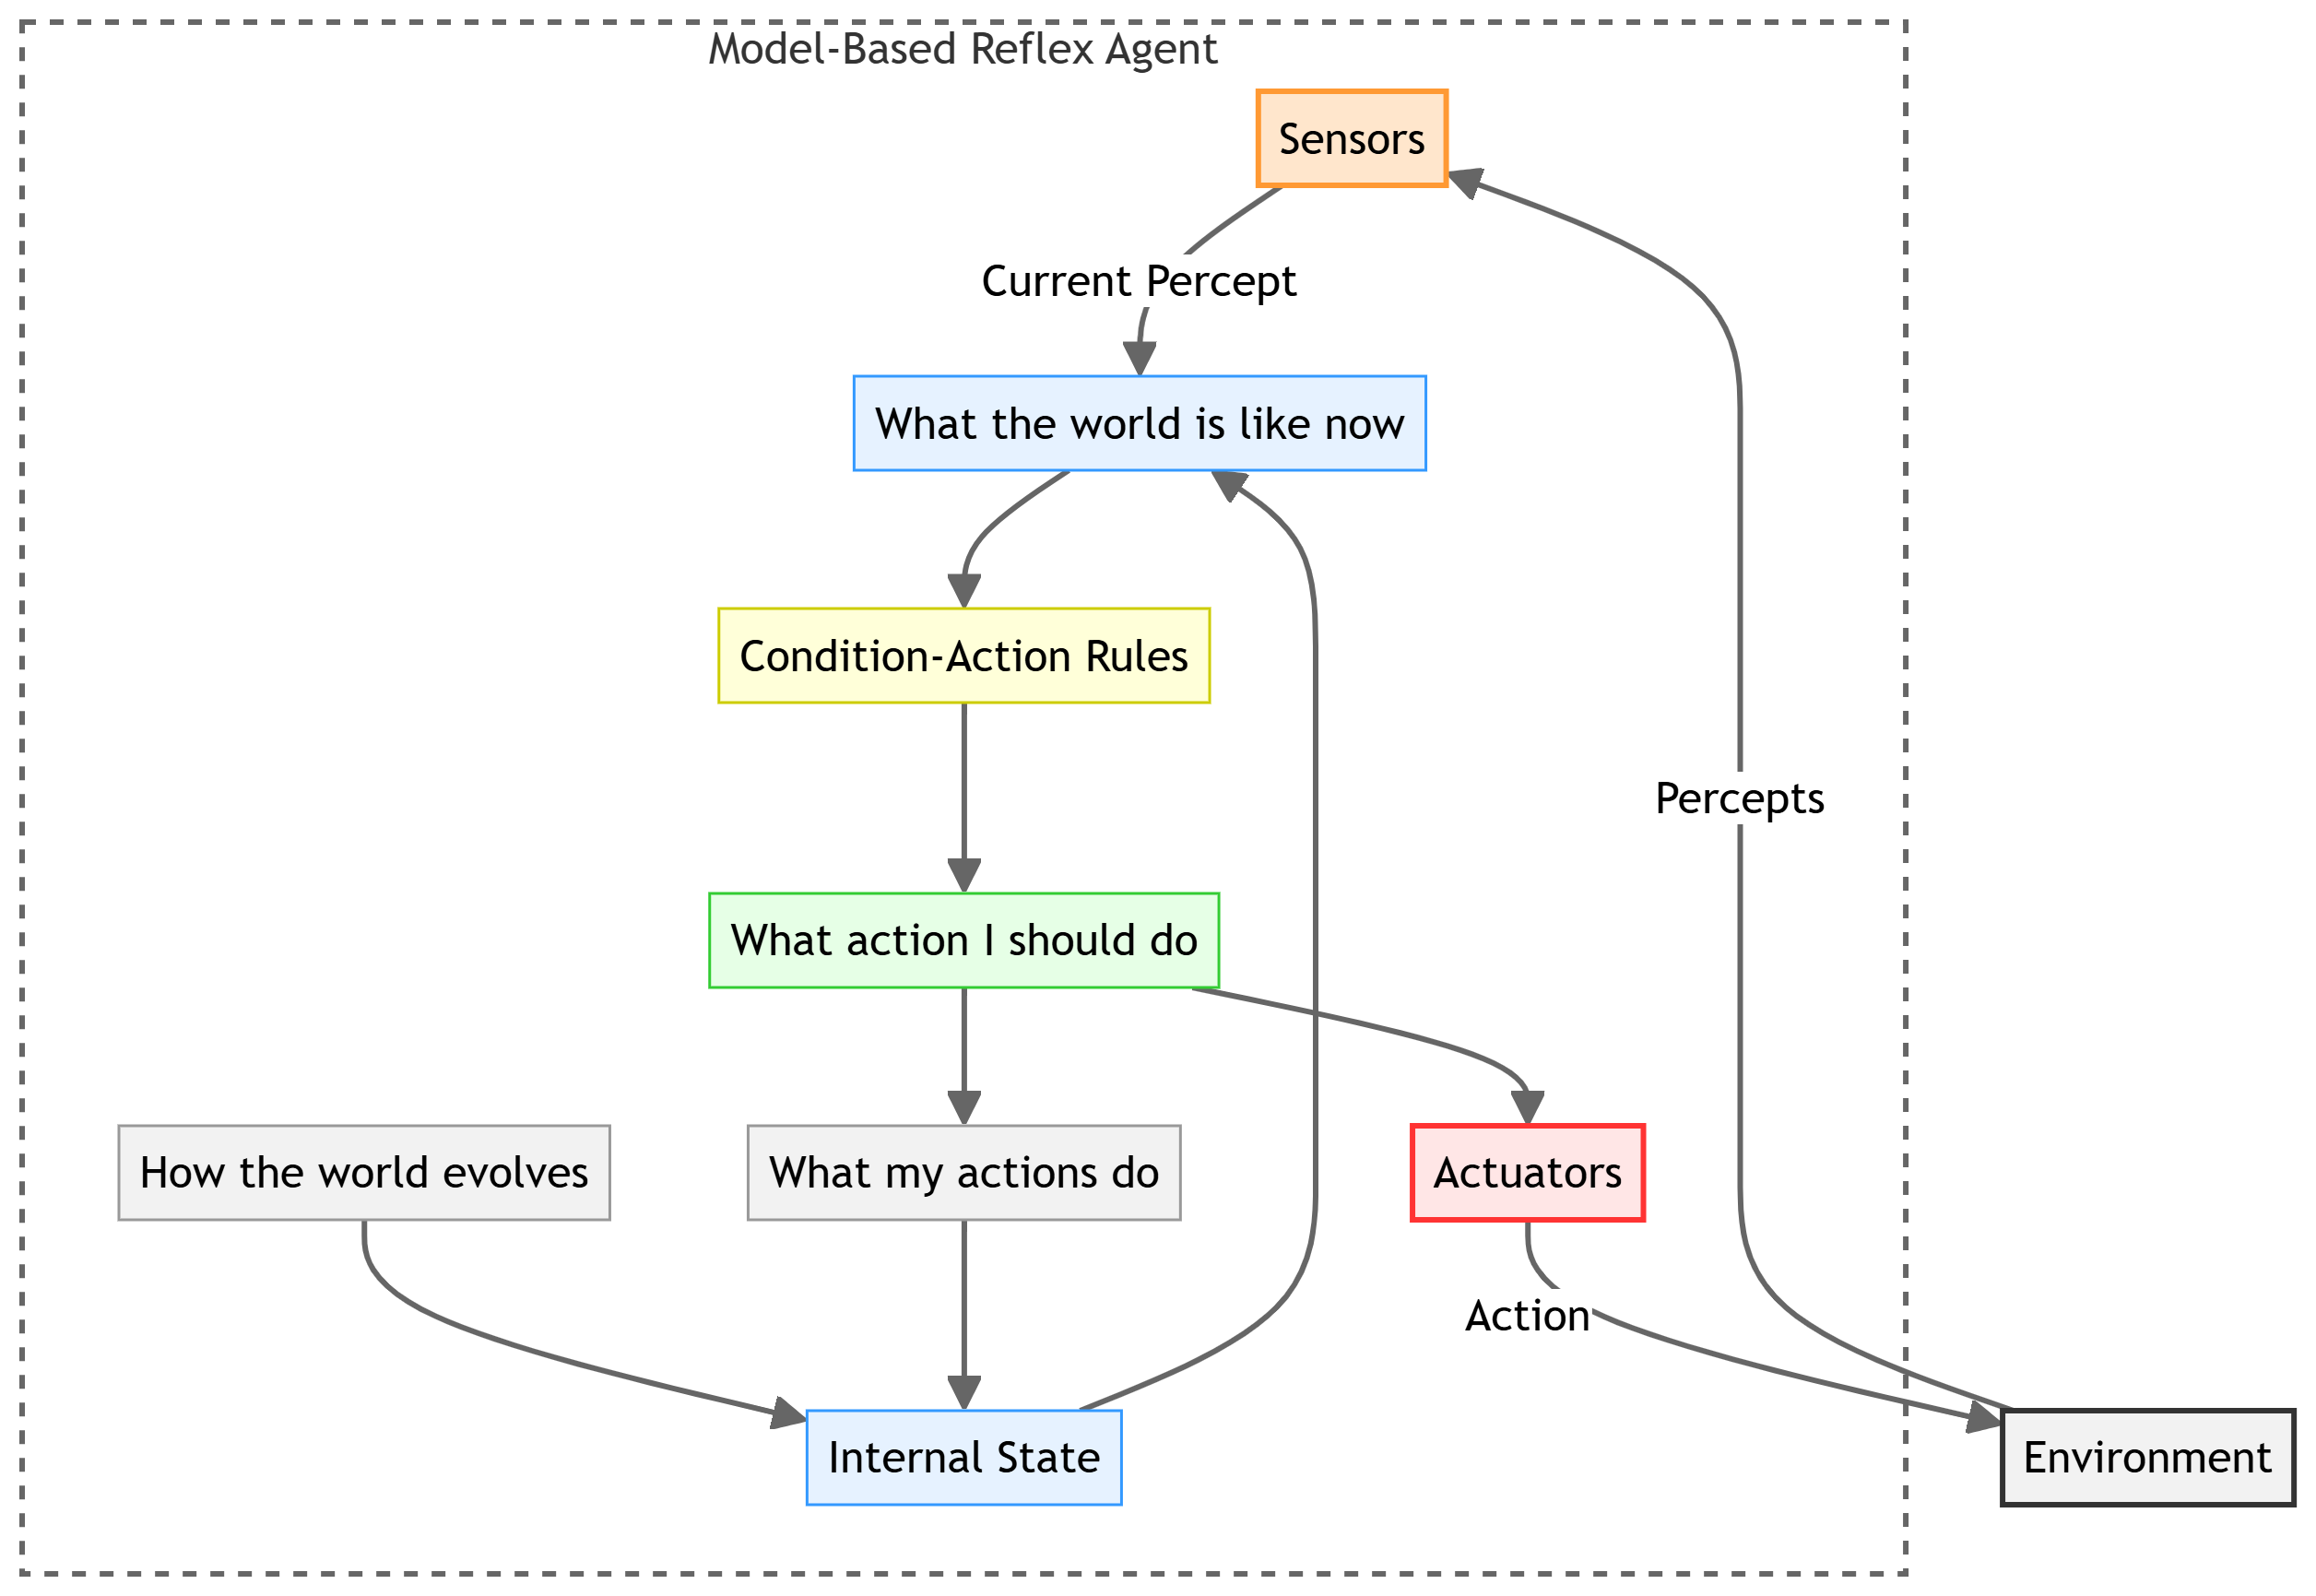
\includegraphics[width=0.75\textwidth,height=0.32\textheight,keepaspectratio]{../Images/chapter_02/model_based_agent.png}
\caption{Model-Based Reflex Agent Structure}
\end{figure}
\begin{enumerate}
  \item \textbf{Learning Agent Architecture:}
\end{enumerate}
    \begin{figure}[H]
\centering
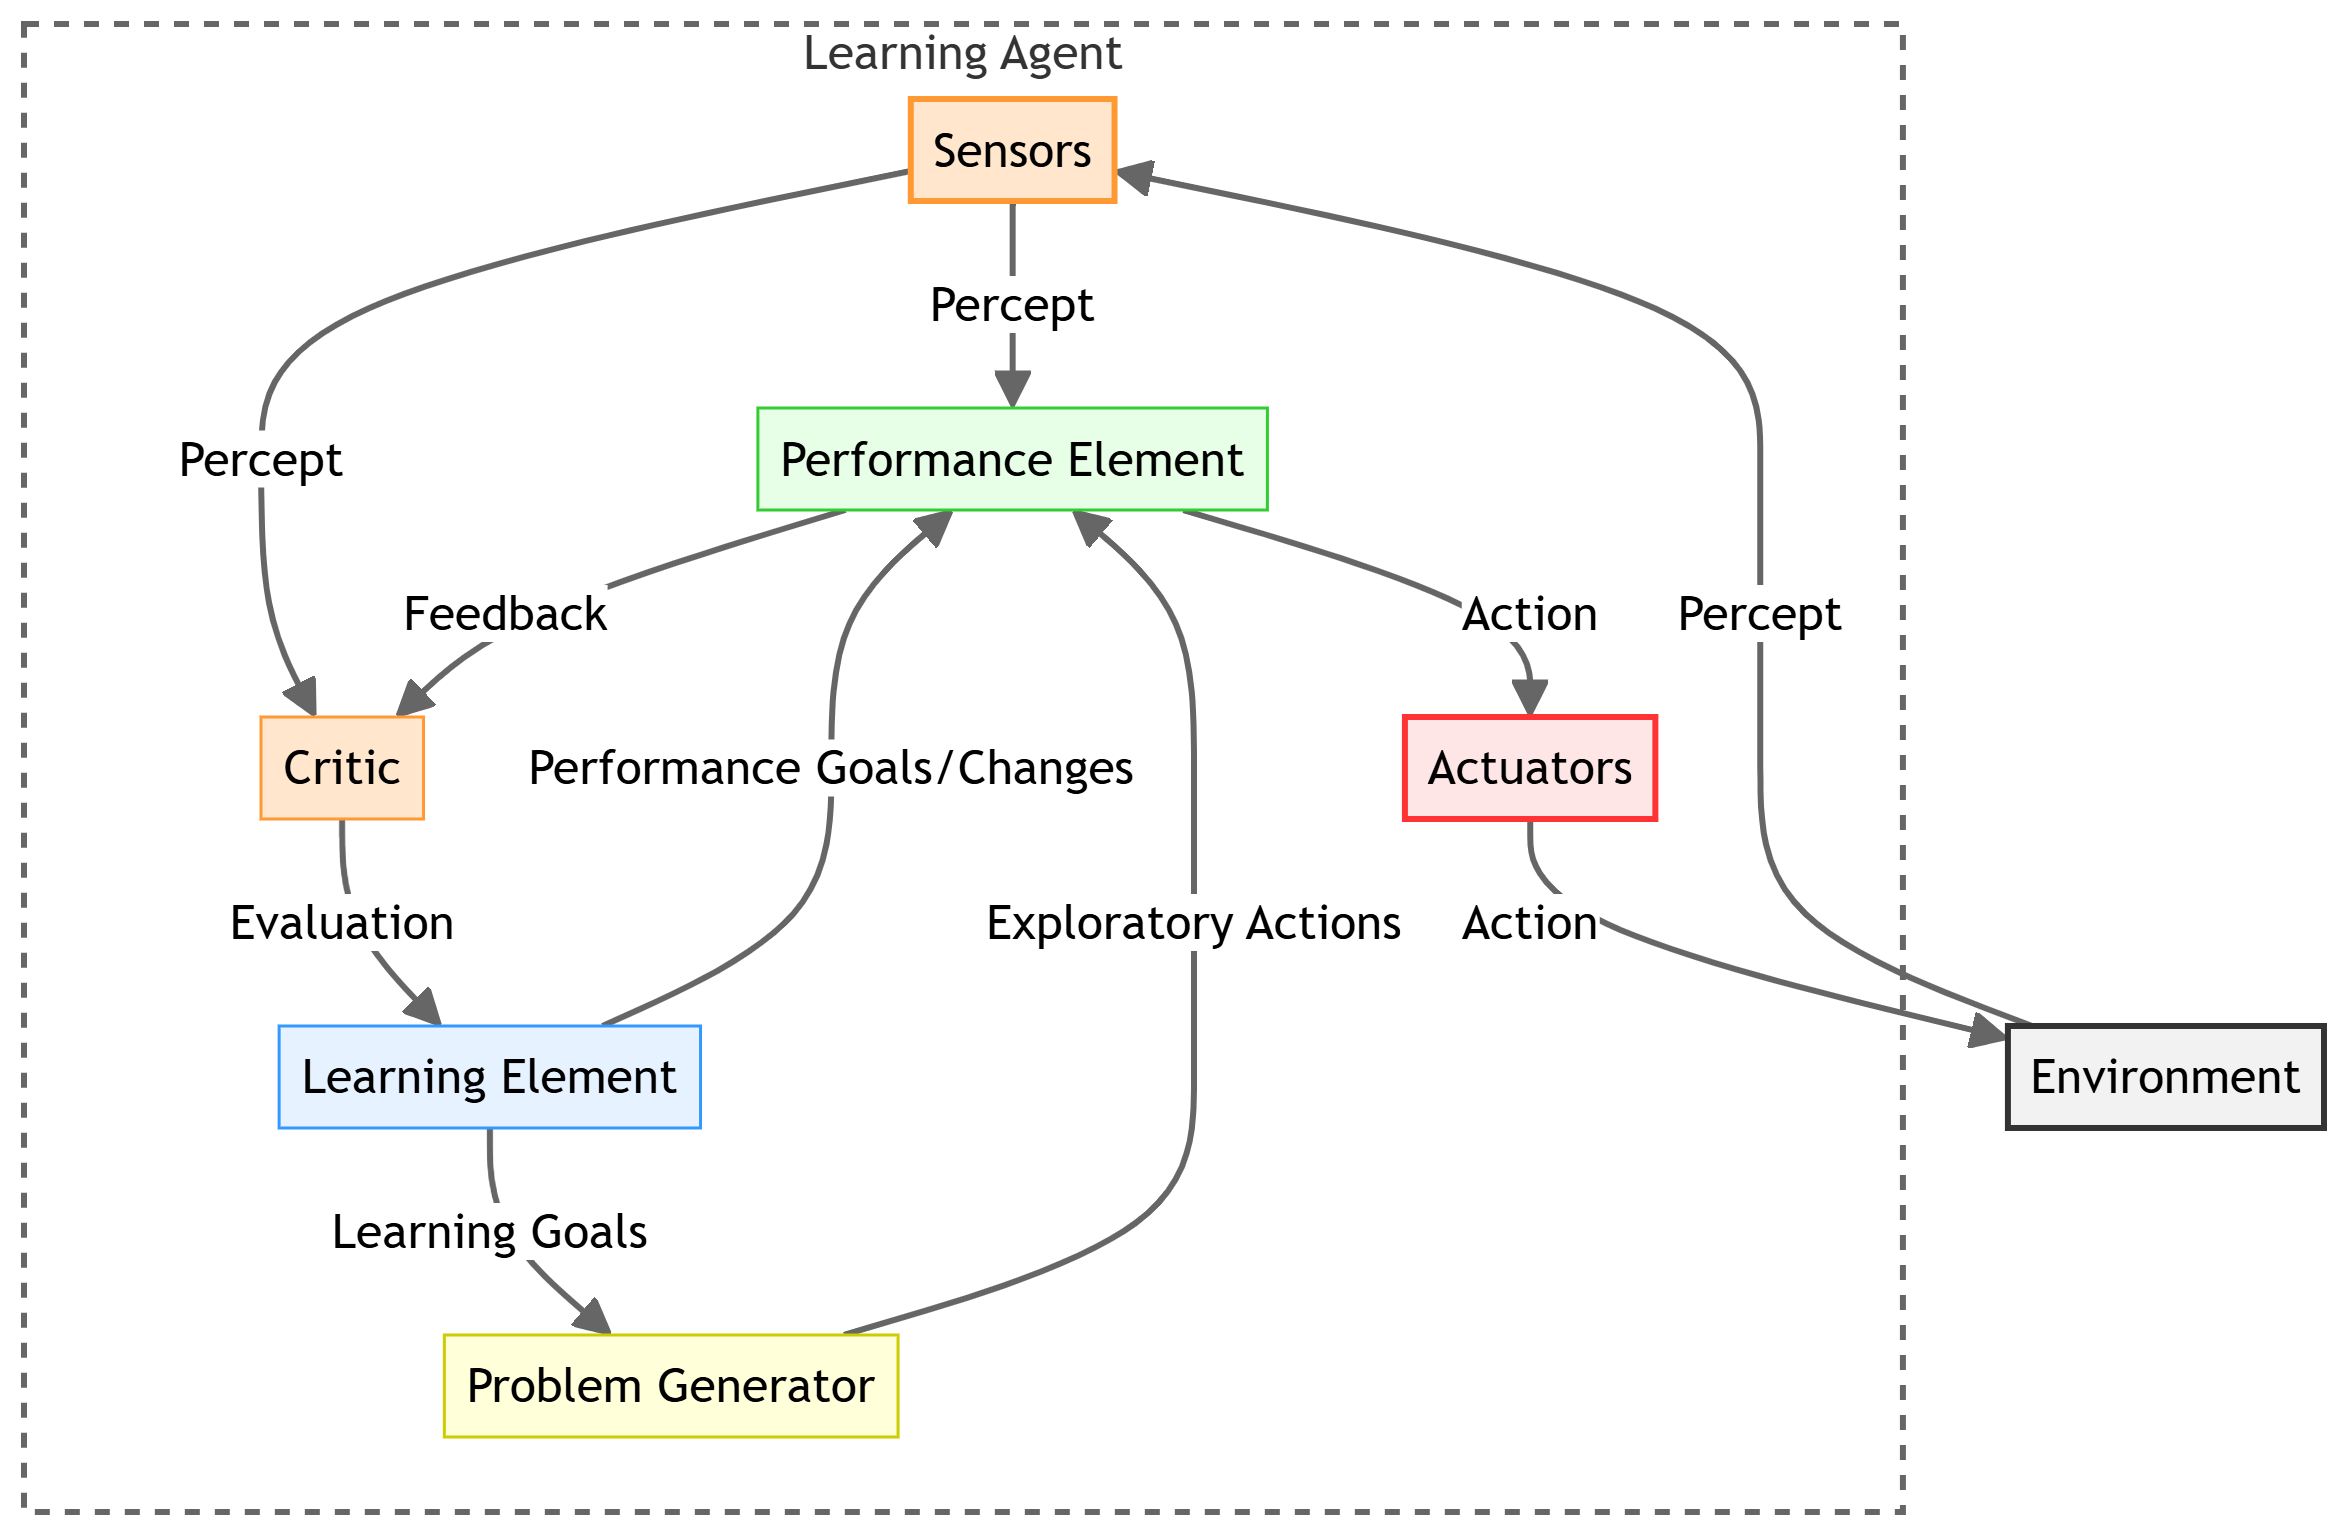
\includegraphics[width=0.75\textwidth,height=0.32\textheight,keepaspectratio]{../Images/chapter_02/learning_agent.png}
\caption{Learning Agent Structure}
\end{figure}

\subsection{One-Line Revision}
\begin{itemize}
  \item   An agent acts using actuators and senses using sensors.
  \item   A simple reflex agent uses current percepts only; model-based reflex agents use internal states to track the unobserved environment.
  \item   Goal-based agents plan to achieve goals; utility-based agents maximize a real-valued performance metric.
  \item   A learning agent separates the critic (evaluator) from the learning element (improver) and the problem generator (explorer).
  \item   Environments can be fully/partially observable, deterministic/stochastic, episodic/sequential, static/dynamic, discrete/continuous, single/multi-agent.
\end{itemize}


\section{Unit III: Solving Problems by Searching (Uninformed Search)}

\subsection{1. Important Definitions}
\begin{itemize}
  \item   \textbf{Uninformed Search (Blind Search):} Search algorithms that do not use any problem-specific knowledge (heuristics) to guide the search process. They only use the problem definition to explore the state space.
  \item   \textbf{State Space:} The set of all possible configurations (states) the problem can be in.
  \item   \textbf{Initial State:} The starting configuration of the problem.
  \item   \textbf{Goal State:} The desired configuration that the search aims to find.
  \item   \textbf{Operators (Successor Function):} Actions that can be applied to a state to transition to a new state.
  \item   \textbf{Path:} A sequence of states from the initial state to a goal state.
  \item   \textbf{Cost:} The cost associated with applying an operator (usually 1 for unweighted graphs).
\end{itemize}

\subsection{2. Characteristics of Uninformed Search}
\begin{itemize}
  \item   \textbf{No Heuristics:} Does not use any problem-specific knowledge to guide the search.
  \item   \textbf{Systematic Exploration:} Explores the state space systematically to find a solution.
  \item   \textbf{Completeness:} Guaranteed to find a solution if one exists (depending on the algorithm).
  \item   \textbf{Optimality:} Guaranteed to find the optimal (lowest cost) solution if one exists (depending on the algorithm).
  \item   \textbf{Memory Usage:} Can be memory-intensive as it may need to store large portions of the state space.
\end{itemize}

\subsection{3. Important Search Algorithms}
\begin{enumerate}
  \item \textbf{Breadth-First Search (BFS):}
\end{enumerate}
\begin{itemize}
  \item   \textbf{Principle:} Explores the state space level by level. It expands all nodes at the current depth before moving to the next depth level. Uses a queue data structure.
  \item   \textbf{Completeness:} Yes, if a solution exists and the branching factor is finite.
  \item   \textbf{Optimality:} Yes, if the cost of each step is uniform (e.g., 1). Finds the shortest path in terms of number of edges.
  \item   \textbf{Time/Space Complexity:} $O(b^d)$, where $b$ is branching factor and $d$ is depth.
\end{itemize}
\begin{enumerate}
  \item \textbf{Depth-First Search (DFS):}
\end{enumerate}
\begin{itemize}
  \item   \textbf{Principle:} Explores as far as possible along each branch before backtracking. Uses a stack data structure.
  \item   \textbf{Completeness:} No, fails in infinite paths or cycles.
  \item   \textbf{Optimality:} No.
  \item   \textbf{Time/Space Complexity:} Time: $O(b^m)$, Space: $O(bm)$ (where $m$ is max depth).
\end{itemize}
\begin{enumerate}
  \item \textbf{Depth-Limited Search (DLS):}
\end{enumerate}
\begin{itemize}
  \item   \textbf{Principle:} DFS with a depth limit $l$ imposed.
\end{itemize}
\begin{enumerate}
  \item \textbf{Iterative Deepening Search (IDDFS):}
\end{enumerate}
\begin{itemize}
  \item   \textbf{Principle:} Performs DLS with increasing limits $l = 0, 1, 2...$ Combines DFS space efficiency $O(bd)$ with BFS completeness and optimality.
\end{itemize}
\begin{enumerate}
  \item \textbf{Uniform Cost Search (UCS):}
\end{enumerate}
\begin{itemize}
  \item   \textbf{Principle:} Expands the node with the lowest path cost $g(n)$ using a priority queue. Optimal for arbitrary step costs.
\end{itemize}

\subsection{4. Algorithm Properties}
\begin{table}[H]
\centering
\begin{tabular}{|p{\dimexpr 0.16666666666666666\textwidth - 2\tabcolsep - 1.5\arrayrulewidth\relax}|p{\dimexpr 0.16666666666666666\textwidth - 2\tabcolsep - 1.5\arrayrulewidth\relax}|p{\dimexpr 0.16666666666666666\textwidth - 2\tabcolsep - 1.5\arrayrulewidth\relax}|p{\dimexpr 0.16666666666666666\textwidth - 2\tabcolsep - 1.5\arrayrulewidth\relax}|p{\dimexpr 0.16666666666666666\textwidth - 2\tabcolsep - 1.5\arrayrulewidth\relax}|p{\dimexpr 0.16666666666666666\textwidth - 2\tabcolsep - 1.5\arrayrulewidth\relax}|}
\hline
Property & BFS & DFS & DLS & IDDFS & UCS \\
\hline
\textbf{Completeness} & Yes & No & No & Yes & Yes \\
\hline
\textbf{Time Complexity} & $O(b^d)$ & $O(b^m)$ & $O(b^l)$ & $O(b^d)$ & $O(b^{1 + \lfloor C^*/\epsilon \rfloor})$ \\
\hline
\textbf{Space Complexity} & $O(b^d)$ & $O(bm)$ & $O(bl)$ & $O(bd)$ & $O(b^{1 + \lfloor C^*/\epsilon \rfloor})$ \\
\hline
\textbf{Optimality} & Yes (uniform) & No & No & Yes (uniform) & Yes \\
\hline
\end{tabular}
\end{table}

\subsection{Diagrams to Practice}
\begin{enumerate}
  \item \textbf{Water Jug Solution Path:}
\end{enumerate}
    \begin{figure}[H]
\centering
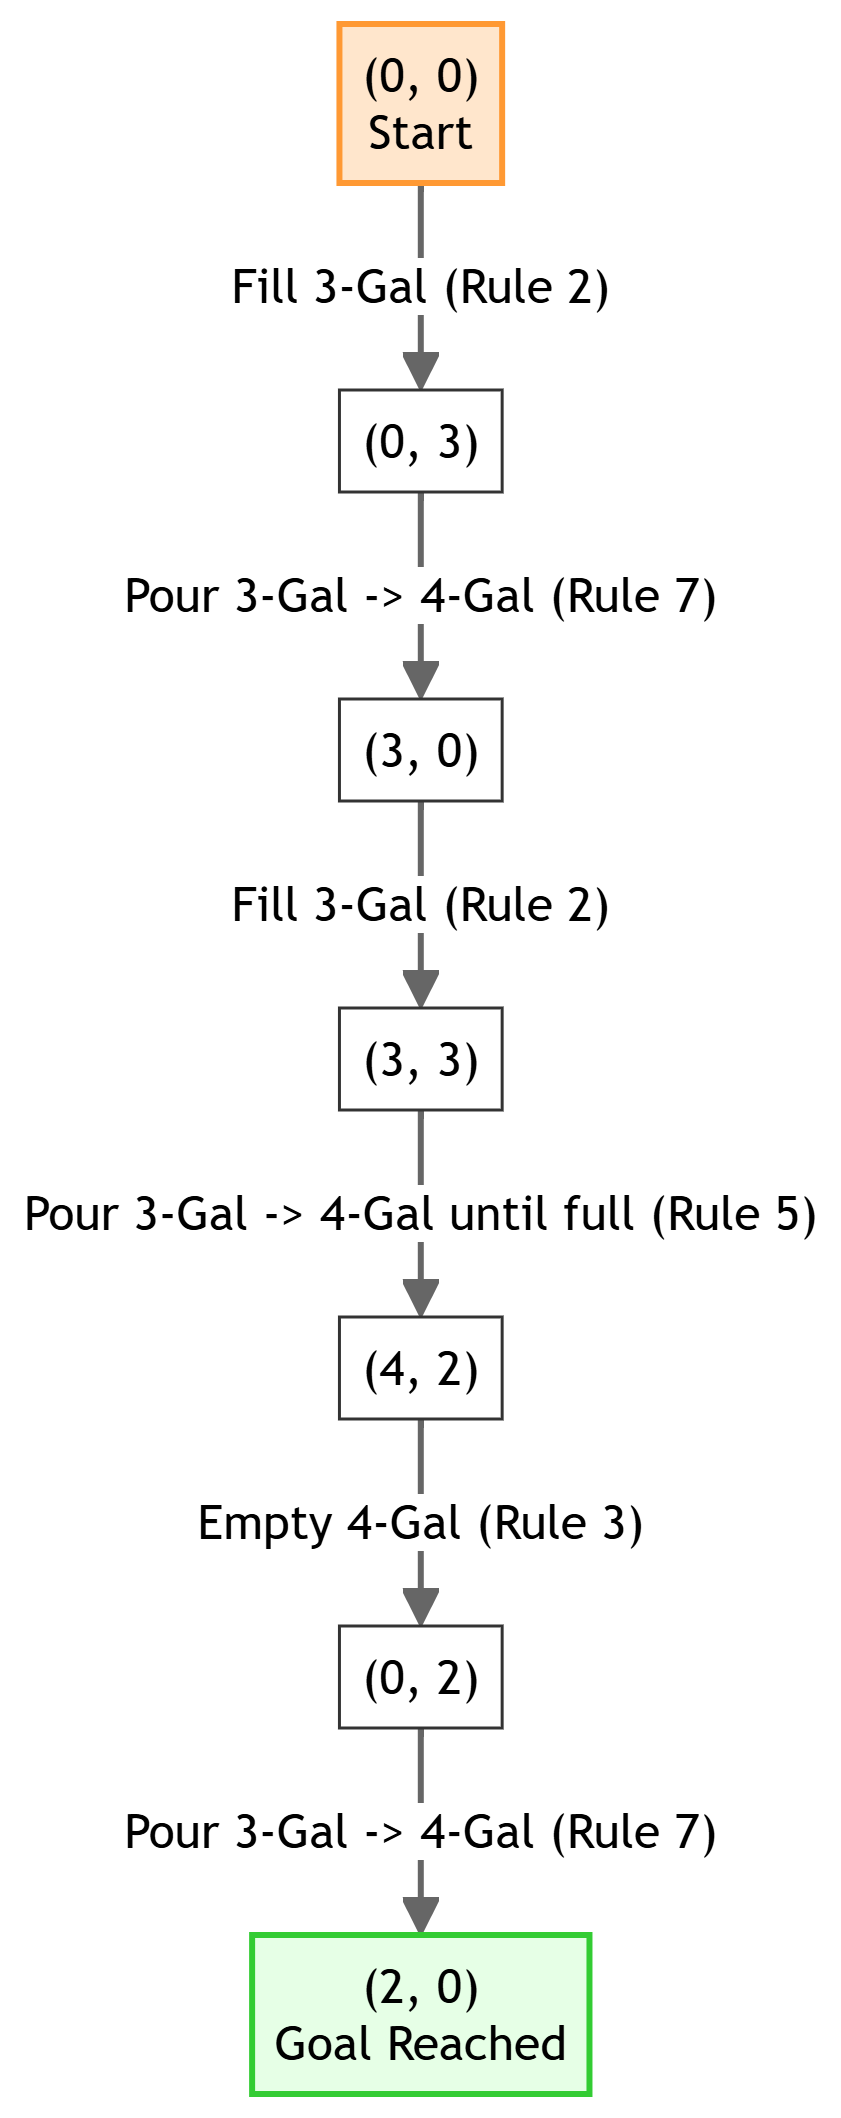
\includegraphics[width=0.75\textwidth,height=0.32\textheight,keepaspectratio]{../Images/chapter_03/water_jug_trace.png}
\caption{Water Jug Traced Solution Path}
\end{figure}


\section{Unit IV: Informed Search \& Exploration}

\subsection{1. Important Definitions}
\begin{itemize}
  \item   \textbf{Informed Search (Heuristic Search):} Search algorithms that use problem-specific knowledge (heuristics) to guide the search process. They use an evaluation function to estimate the cost from the current state to the goal state.
  \item   \textbf{Heuristic Function ($h(n)$):} An informed guess about the cost from the current state to the goal state. It is used to guide the search process.
  \item   \textbf{Evaluation Function ($f(n)$):} A function that evaluates the cost of a state. It is used to guide the search process.
  \item   \textbf{Recursive Best-First Search (RBFS):} An optimal, best-first heuristic search algorithm that runs in linear space ($O(bd)$) by using recursive depth-first execution and maintaining an $f$-limit value for backtracking.
\end{itemize}

\subsection{2. Important Algorithms}
\begin{enumerate}
  \item \textbf{Greedy Best-First Search:}
\end{enumerate}
\begin{itemize}
  \item   \textbf{Principle:} Expands the node that appears to be closest to the goal state, as estimated by the heuristic function.
  \item   \textbf{Evaluation Function:} $f(n) = h(n)$
  \item   \textbf{Completeness/Optimality:} No.
\end{itemize}
\begin{enumerate}
  \item \textbf{A* Search:}
\end{enumerate}
\begin{itemize}
  \item   \textbf{Principle:} Expands the node that appears to be closest to the goal state, as estimated by the evaluation function $f(n)$.
  \item   \textbf{Evaluation Function:} $f(n) = g(n) + h(n)$, where $g(n)$ is the cost from the start state to the current state, and $h(n)$ is the estimated cost from the current state to the goal state.
  \item   \textbf{Completeness/Optimality:} Yes, if $h(n)$ is admissible (tree search) or consistent (graph search).
\end{itemize}
\begin{enumerate}
  \item \textbf{Local Search and Optimization Techniques:}
\end{enumerate}
\begin{itemize}
  \item   \textbf{Hill-Climbing Search:} Greedy algorithm that moves to the neighboring state with the highest heuristic value. Fails at local maxima, ridges, and plateaus.
  \item   \textbf{Local Beam Search:} Tracks $k$ states instead of just one, expanding all successors and keeping the best $k$.
\end{itemize}
    \textit{   \textbf{AO} Search:} Used for search trees representing AND-OR graphs (decomposable problems).

\subsection{Diagrams to Practice}
\begin{enumerate}
  \item \textbf{Heuristic Consistency Triangle:}
\end{enumerate}
    \begin{figure}[H]
\centering
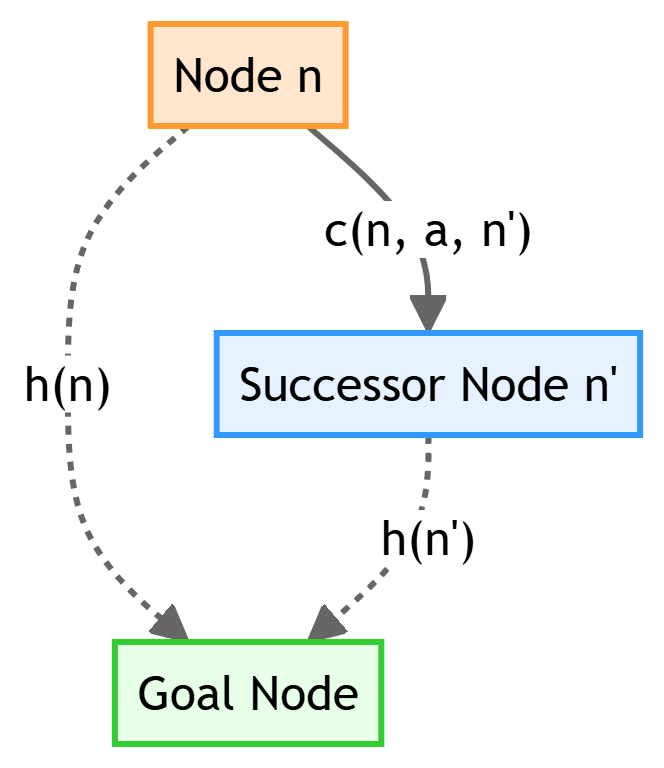
\includegraphics[width=0.75\textwidth,height=0.32\textheight,keepaspectratio]{../Images/chapter_04/consistency_triangle.png}
\caption{Heuristic Consistency Inequality Triangle}
\end{figure}
\begin{enumerate}
  \item \textbf{AND-OR Graph Decompositions:}
\end{enumerate}
    \begin{figure}[H]
\centering
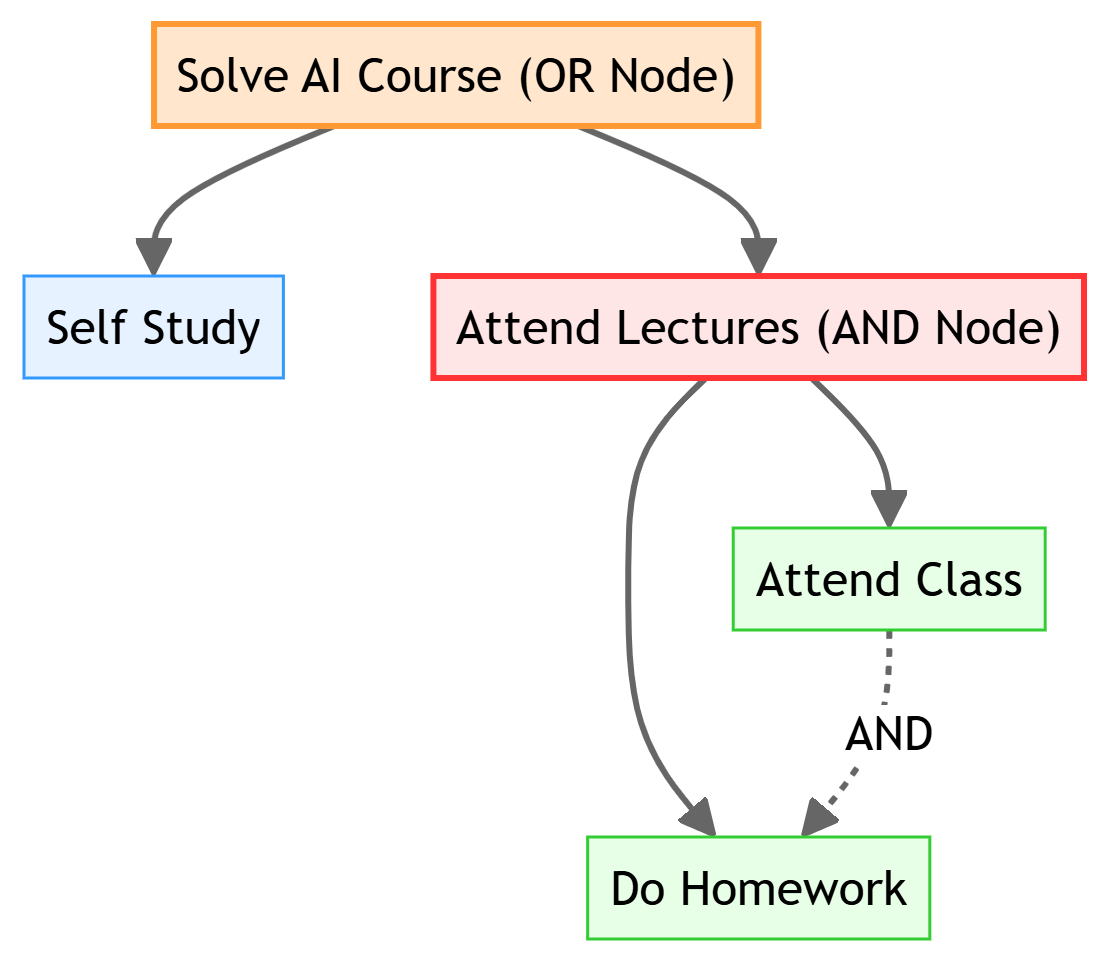
\includegraphics[width=0.75\textwidth,height=0.32\textheight,keepaspectratio]{../Images/chapter_04/and_or_graph.png}
\caption{AND-OR Graph Decompositions}
\end{figure}

\subsection{One-Line Revision}
\begin{itemize}
  \item   Greedy Best-First Search evaluates nodes using $f(n) = h(n)$, expanding the node estimated to be closest to the goal.
  \item   The space complexity of Greedy Search is exponential ($O(b^l)$) because it stores all frontier nodes.
  \item   RBFS reduces the space complexity to linear ($O(bd)$) but can have exponential time complexity due to node regeneration.
\end{itemize}


\section{Unit V: Constraint Satisfaction Problems}

\subsection{1. Important Definitions}
\begin{itemize}
  \item   \textbf{Constraint Satisfaction Problem (CSP):} A problem defined by a set of variables, domains (allowed values), and constraints restricting value combinations.
  \item   \textbf{Backtracking Search:} DFS-based search for CSPs where variables are assigned sequentially and reverted on constraint violation.
  \item   \textbf{Alldifferent Constraint:} A global constraint specifying that all variables in a set must be assigned unique values.
  \item   \textbf{Flexible CSP:} A CSP formulation where constraints are relaxed (preferences/soft constraints) to allow a solution when the problem is overconstrained.
\end{itemize}

\subsection{Frequently Asked Questions}
\begin{enumerate}
  \item \textbf{"Solve the cryptarithmetic problem: SEND + MORE = MONEY." [15M][]}
\end{enumerate}
    \textit{   }Core point:* Set up variables, domains, and column carry constraints. Solve sequentially: $M=1$ (carry), $O=0$, $S=9$, $C_3=0$, $C_2=1$, $N=E+1$. Find remaining digits: $R=7$, $E=5$, $N=6$, $D=8$, $Y=3$.

\subsection{Diagrams to Practice}
\begin{enumerate}
  \item \textbf{Australia Constraint Graph:}
\end{enumerate}
    \begin{figure}[H]
\centering
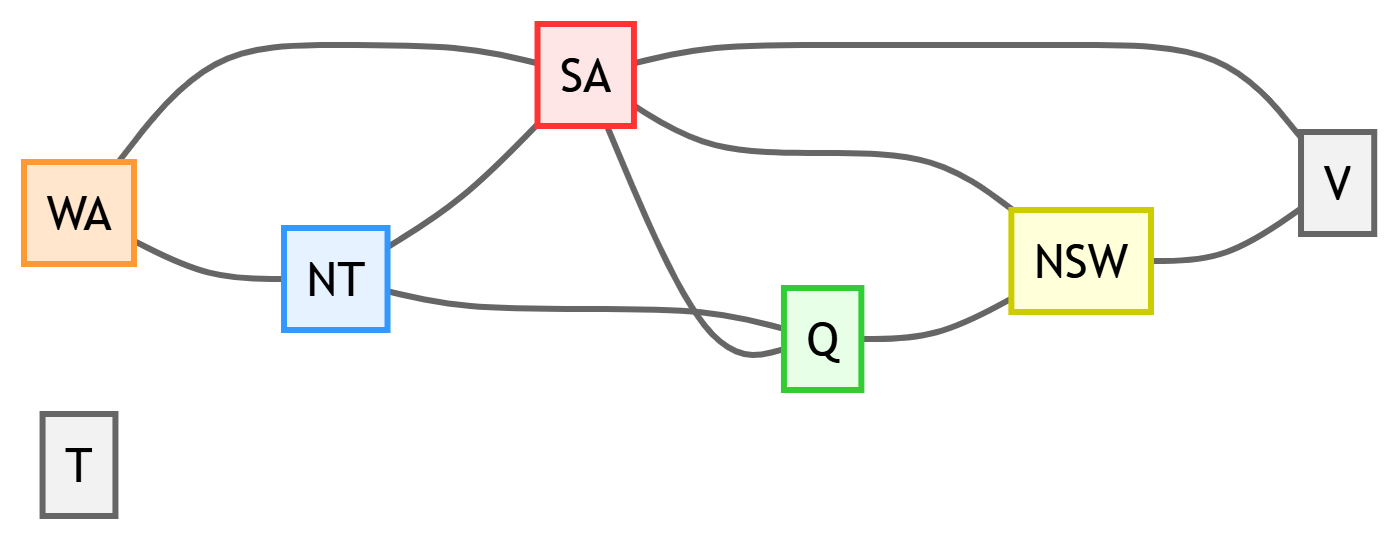
\includegraphics[width=0.75\textwidth,height=0.32\textheight,keepaspectratio]{../Images/chapter_05/australia_map.png}
\caption{Australia Map-Coloring Outline}
\end{figure}

\subsection{One-Line Revision}
\begin{itemize}
  \item   CSPs use a factored state representation (variables and constraints) instead of atomic black boxes.
  \item   Backtracking is the standard complete search algorithm for CSPs.
  \item   Flexible CSPs relax constraints to handle overconstrained problems.
  \item   Backtracking search is structurally based on a LIFO stack and recursion, and Prolog is a standard programming language for Constraint Programming.
\end{itemize}



\section{Unit VI: Adversarial Search}

\subsection{1. Important Definitions}
\begin{itemize}
  \item   \textbf{Adversarial Search:} Search algorithms used in competitive, multi-agent environments (games).
  \item   \textbf{Minimax Algorithm:} A recursive algorithm that calculates optimal moves in zero-sum games by maximizing for MAX and minimizing for MIN.
  \item   \textbf{Alpha-Beta Pruning:} An optimization that skips evaluating subtrees that cannot possibly affect the final minimax decision.
\end{itemize}
    \textit{   }Alpha ($\alpha$):* The best (highest) utility value found so far for MAX.
    \textit{   }Beta ($\beta$):* The best (lowest) utility value found so far for MIN.

\subsection{Frequently Asked Questions}
\begin{enumerate}
  \item \textbf{"Explain Alpha-Beta Pruning with a trace." [15M][]}
\end{enumerate}
    \textit{   }Core point:* Explain $\alpha$ and $\beta$. Prune branches whenever $\beta \le \alpha$ (alpha-cutoff at MIN node, beta-cutoff at MAX node). Show a sample tree with leaf evaluations and marked cutoffs.

\subsection{Diagrams to Practice}
\begin{enumerate}
  \item \textbf{Pruned Game Tree:}
\end{enumerate}
    \begin{figure}[H]
\centering
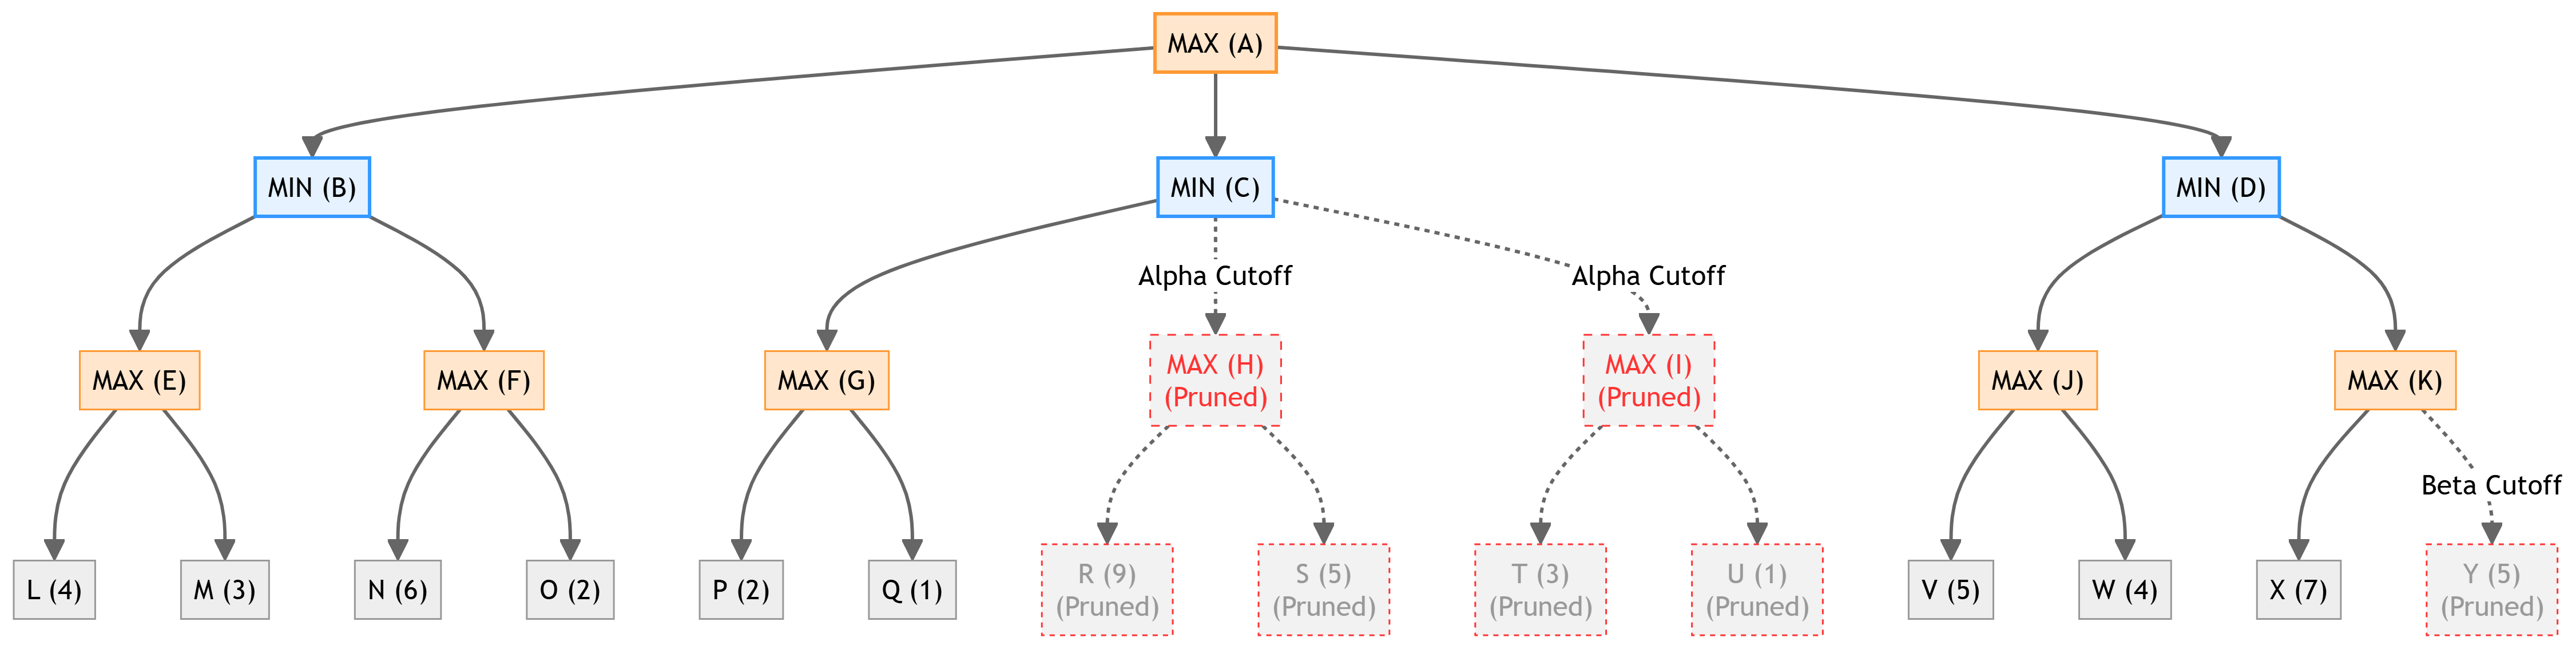
\includegraphics[width=0.75\textwidth,height=0.32\textheight,keepaspectratio]{../Images/chapter_06/alphabeta_tree.png}
\caption{Alpha-Beta Pruning Game Tree}
\end{figure}

\subsection{One-Line Revision}
\begin{itemize}
  \item   Standard minimax has time complexity $O(b^d)$, which is reduced to $O(b^{d/2})$ with perfect alpha-beta pruning.
  \item   Pruning does not change the optimal move selection; it only speeds up the search.
\end{itemize}


\section{Unit VII: Logical Agents}

\subsection{1. Important Definitions}
\begin{itemize}
  \item   \textbf{Propositional Logic:} A logic system dealing with propositions (T/F statements) and connectives ($\land, \lor, \neg, \rightarrow, \leftrightarrow$).
  \item   \textbf{Soundness:} An inference rule is sound if it only derives true sentences from true premises.
  \item   \textbf{Completeness:} An inference rule is complete if it can derive all sentences entailed by the premises.
  \item   \textbf{Tautology:} A sentence that is True under all truth assignments (e.g., Peirce's Law: $(((P \rightarrow Q) \rightarrow P) \rightarrow P)$).
  \item   \textbf{Modus Ponens:} Inference rule of form: $\frac{P, \quad P \rightarrow Q}{Q}$.
  \item   \textbf{Modus Tollens:} Inference rule of form: $\frac{\neg Q, \quad P \rightarrow Q}{\neg P}$.
  \item   \textbf{Unit Clause:} A clause containing exactly a single literal (e.g. $P$ or $\neg Q$).
  \item   \textbf{Proposition Symbol (AI Constants):} In AI, the two standard logical constant symbols representing fixed truth values: \textbf{True} ($\top$) and \textbf{False} ($\bot$).
  \item   \textbf{Validity \& Satisfiability:} A sentence is valid if it is true in all models (Tautology). A sentence is satisfiable if it is true in at least one model; if a sentence has no model where it is true, it is unsatisfiable (Contradiction).
\end{itemize}

\subsection{Frequently Asked Questions}
\begin{enumerate}
  \item \textbf{"Prove that Peirce's Law is a Tautology." [5M][]}
\end{enumerate}
    \textit{   }Core point:* Construct a 4-row truth table for $P, Q$. Compute column-wise: $P \rightarrow Q$, $(P \rightarrow Q) \rightarrow P$, and the final implication, proving all rows are True.
\begin{enumerate}
  \item \textbf{"Explain Wumpus World environment." [10M][]}
\end{enumerate}
    \textit{   }Core point:* State PEAS components. Show how Breeze maps to Pit and Stench to Wumpus, and trace safety reasoning.

\subsection{Diagrams to Practice}
\begin{enumerate}
  \item \textbf{Wumpus World Grid:}
\end{enumerate}
    \begin{figure}[H]
\centering
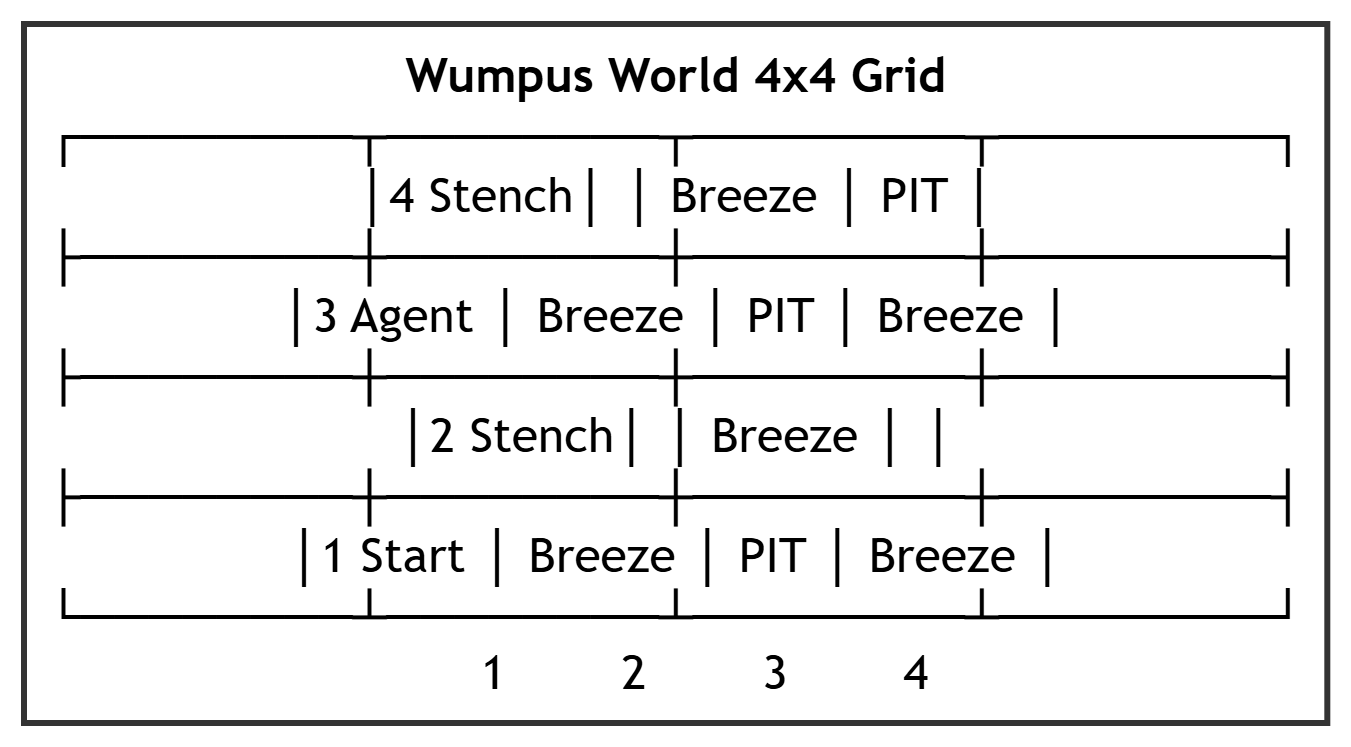
\includegraphics[width=0.75\textwidth,height=0.32\textheight,keepaspectratio]{../Images/chapter_07/wumpus_world_grid.png}
\caption{Wumpus World Grid Layout}
\end{figure}

\subsection{One-Line Revision}
\begin{itemize}
  \item   Knowledge-based agents query the KB with `ASK` and insert facts/percepts with `TELL`.
  \item   Propositional logic is monotonic but lacks variables and quantifiers.
  \item   Every sentence of propositional logic can be converted to an inferred equivalent CNF sentence. If the CNF is unsatisfiable, the original statement is unsatisfiable.
  \item   Resolution is a single inference rule because it is refutation-complete, meaning no other rules (like Modus Ponens) are required to compute logical entailment.
  \item   There are exactly 2 constant proposition symbols in AI logic: True and False.
\end{itemize}


\section{Unit VIII: First-Order Logic \& Knowledge Representation}

\subsection{1. Important Definitions}
\begin{itemize}
  \item   \textbf{First-Order Logic (FOL):} Logic system representing objects, properties, relations, and quantifiers ($\forall, \exists$).
  \item   \textbf{Horn Clause:} A clause containing at most one positive literal. Basis of PROLOG.
  \item   \textbf{Skolemisation:} Eliminating existential quantifiers by replacing them with unique constants or functions (when inside universal scopes).
  \item   \textbf{Semantic Network:} A graph with concept nodes and directed, labeled relation edges.
  \item   \textbf{Fuzzy Logic:} A multi-valued logic representing degrees of membership in a set using real numbers in $[0, 1]$.
\end{itemize}

\subsection{Frequently Asked Questions}
\begin{enumerate}
  \item \textbf{"Convert a FOL formula into Clausal Form (CNF)." [15M][]}
\end{enumerate}
    \textit{   }Core point:* Follow the 7 steps: eliminate implications, move negations inward, standardize variables, Skolemise, drop $\forall$, distribute $\lor$ over $\land$, isolate clauses.
\begin{enumerate}
  \item \textbf{"Prove Marcus hated Caesar using Resolution Refutation." [15M][]}
\end{enumerate}
    \textit{   }Core point:* Translate statements into FOPL clauses. Negate the goal ($\neg Hate(Marcus, Caesar)$). Apply resolution to derive the empty clause ($\Box$).

\subsection{Diagrams to Practice}
\begin{enumerate}
  \item \textbf{Semantic Net Diagram:}
\end{enumerate}
    \begin{figure}[H]
\centering
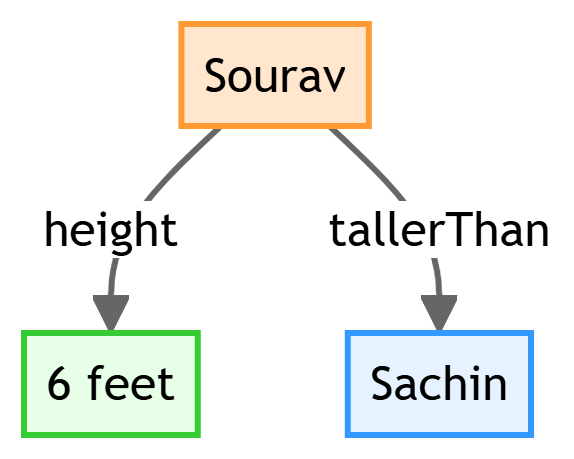
\includegraphics[width=0.75\textwidth,height=0.32\textheight,keepaspectratio]{../Images/chapter_08/semantic_network.png}
\caption{Semantic Network}
\end{figure}
\begin{enumerate}
  \item \textbf{Resolution Refutation Proof Tree:}
\end{enumerate}
    \begin{figure}[H]
\centering
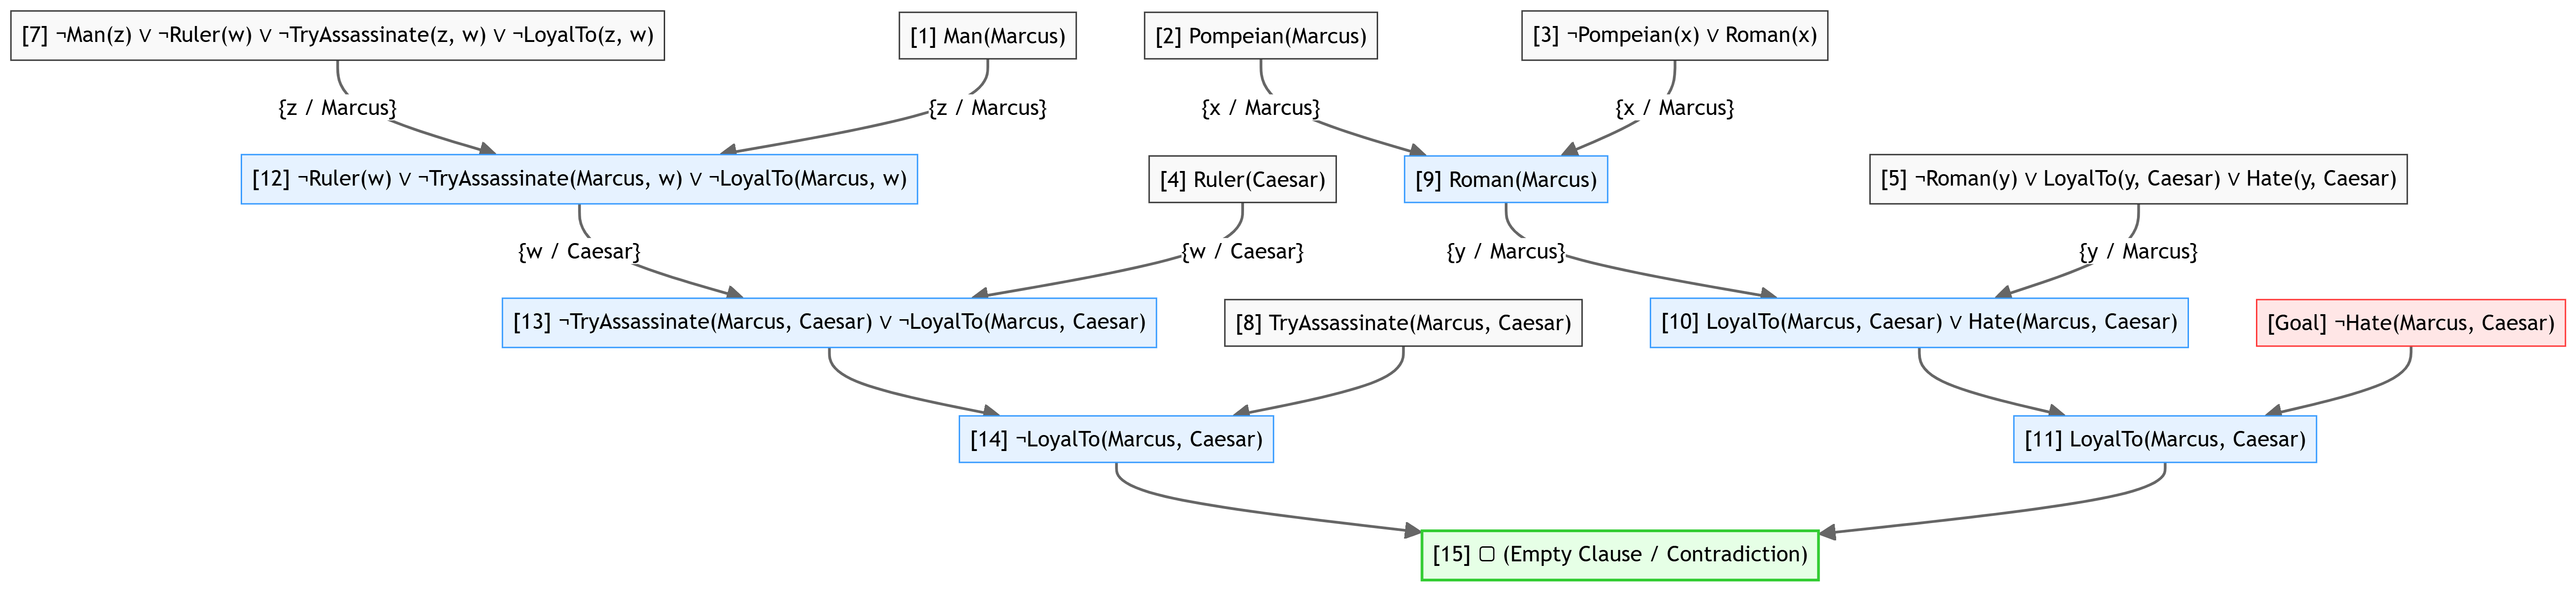
\includegraphics[width=0.75\textwidth,height=0.32\textheight,keepaspectratio]{../Images/chapter_08/resolution_steps.png}
\caption{Resolution Refutation Proof Tree}
\end{figure}

\subsection{One-Line Revision}
\begin{itemize}
  \item   Fuzzy union uses $\max$ and intersection uses $\min$ of membership functions.
  \item   Hebbian learning in NN adjusts weights according to $\Delta w_{ij} = \eta a_i a_j$.
  \item   Genetic algorithms search using populations, selection, crossover, and mutation.
\end{itemize}


\section{Solved Exam One-Liners (CA4 Database)}

\begin{itemize}
  \item   \textbf{Q35. Which are needed to compute the logical inference algorithm?}
\end{itemize}
    \textit{   }Answer:* \textbf{Validity, Satisfiability, and Logical equivalence} (All of the mentioned)
\begin{itemize}
  \item   \textbf{Q36. Which search method will expand the node that is closest to the goal?}
\end{itemize}
    \textit{   }Answer:* \textbf{Greedy best-first search} (evaluates using $f(n) = h(n)$)
\begin{itemize}
  \item   \textbf{Q37. Which search uses the problem specific knowledge beyond the definition of the problem?}
\end{itemize}
    \textit{   }Answer:* \textbf{Informed search} (or Heuristic search)
\begin{itemize}
  \item   \textbf{Q38. Backtracking is based on which data structure and algorithm mechanics?}
\end{itemize}
    \textit{   }Answer:* \textbf{Last-In, First-Out (LIFO) stack and Recursion} (Both)
\begin{itemize}
  \item   \textbf{Q39. How many proposition symbols are there in artificial intelligence logic?}
\end{itemize}
    \textit{   }Answer:* \textbf{2} (representing the constant truth symbols \textbf{True} and \textbf{False})
\begin{itemize}
  \item   \textbf{Q40. Which sentences can be converted to inferred equivalent CNF sentences?}
\end{itemize}
    \textit{   }Answer:* \textbf{Every sentence of propositional logic}
\begin{itemize}
  \item   \textbf{Q41. What can be viewed as a single literal of disjunction?}
\end{itemize}
    \textit{   }Answer:* \textbf{Unit clause}
\begin{itemize}
  \item   \textbf{Q42. Uninformed search strategies are better than informed search strategies.}
\end{itemize}
    \textit{   }Answer:* \textbf{False} (informed searches use heuristics to dramatically reduce search space)
\begin{itemize}
  \item   \textbf{Q43. Which values are independent in minimax search algorithm?}
\end{itemize}
    \textit{   }Answer:* \textbf{Pruned leaves x and y} (their values do not affect the root decision)
\begin{itemize}
  \item   \textbf{Q44. Which sentence will be unsatisfiable if the CNF sentence is unsatisfiable?}
\end{itemize}
    \textit{   }Answer:* \textbf{Original statement}
\textit{   \textbf{Q45. The A} algorithm is based on which search strategy?}
    \textit{   }Answer:* \textbf{Best-First Search} (using evaluation function $f(n) = g(n) + h(n)$)
\begin{itemize}
  \item   \textbf{Q46. Flexible CSPs relax on which component of the problem?}
\end{itemize}
    \textit{   }Answer:* \textbf{Constraints} (soft constraints/preferences are relaxed to resolve overconstrained scenarios)
\begin{itemize}
  \item   \textbf{Q47. Which is used to compute the truth of any sentence?}
\end{itemize}
    \textit{   }Answer:* \textbf{Semantics of propositional logic} (evaluates truth values in a model)
\begin{itemize}
  \item   \textbf{Q48. Preparing a schedule for a class of students is what type of problem?}
\end{itemize}
    \textit{   }Answer:* \textbf{CSP (Constraint Satisfaction Problem)}
\begin{itemize}
  \item   \textbf{Q49. Which search is complete and optimal when the heuristic $h(n)$ is consistent?}
\end{itemize}
    \textit{   }Answer:\textit{ \textbf{A} search} (optimal for graph search with consistent heuristics)
\begin{itemize}
  \item   \textbf{Q50. The Heuristic function $h(n)$ represents: \_\_\_\_\_\_\_.}
\end{itemize}
    \textit{   }Answer:* \textbf{Estimated cost of the cheapest path from the current node to the goal node}
\begin{itemize}
  \item   \textbf{Q51. Which form is called a conjunction of disjunction of literals?}
\end{itemize}
    \textit{   }Answer:* \textbf{Conjunctive Normal Form (CNF)}
\begin{itemize}
  \item   \textbf{Q52. What is the space complexity of Greedy best-first search?}
\end{itemize}
    \textit{   }Answer:* \textbf{$O(b^l)$} (or $O(b^m)$), which is exponential in the worst case
\begin{itemize}
  \item   \textbf{Q53. Which inference rule is also called a single inference rule?}
\end{itemize}
    \textit{   }Answer:* \textbf{Resolution} (refutation-complete rule)
\begin{itemize}
  \item   \textbf{Q54. Which of the following problems can be modeled as a CSP?}
\end{itemize}
    \textit{   }Answer:* \textbf{8-Puzzle, Map coloring, and 8-Queen problems} (All of the mentioned)
\begin{itemize}
  \item   \textbf{Q55. Which search uses only linear space for searching?}
\end{itemize}
    \textit{   }Answer:\textit{ \textbf{Recursive Best-First Search (RBFS)} (uses $O(bd)$ space, unlike A}'s exponential space)
\begin{itemize}
  \item   \textbf{Q56. Constraint satisfaction problems on finite domains are typically solved using: \_\_\_\_\_\_\_.}
\end{itemize}
    \textit{   }Answer:* \textbf{Search Algorithms} (specifically Backtracking Search)
\begin{itemize}
  \item   \textbf{Q57. The search strategy that uses problem-specific knowledge is known as: \_\_\_\_\_\_\_.}
\end{itemize}
    \textit{   }Answer:* \textbf{Informed Search} (or Heuristic Search)
\begin{itemize}
  \item   \textbf{Q58. Best-First search can be implemented using which data structure?}
\end{itemize}
    \textit{   }Answer:* \textbf{Priority Queue} (keeps frontier sorted by evaluation function $f(n)$)
\begin{itemize}
  \item   \textbf{Q59. Which programming language is used for Constraint Programming?}
\end{itemize}
    \textit{   }Answer:* \textbf{Prolog} (with specialized CLP(FD) constraint solver libraries)